\documentclass[11pt,a4paper]{article}
\usepackage{iftex}
\ifXeTeX\usepackage{fontspec}\else\usepackage[T1]{fontenc}\usepackage[utf8]{inputenc}\fi
\usepackage[french]{babel}
\ifXeTeX\usepackage{microtype}\else\usepackage{lmodern,microtype}\fi
\usepackage[margin=2.2cm]{geometry}
\usepackage{amsmath,amssymb}
\usepackage{graphicx,booktabs,float,caption,enumitem,xcolor}
\usepackage[hidelinks]{hyperref}
\usepackage{textcomp,newunicodechar}
\newunicodechar{→}{\ensuremath{\rightarrow}}
\newunicodechar{€}{\texteuro}
\newunicodechar{×}{\ensuremath{\times}}
\graphicspath{{../figures/}}
\setlist{itemsep=1pt,topsep=3pt}
\captionsetup{font=small,labelfont=bf}

\title{\textbf{Acheter, rester neutre ou vendre le Nikkei 225 ?}\\[2pt]
\large Un signal mensuel tiré des news et des marchés, pour un investisseur en euros}
\author{Applied ML: Foundations, Engineering \& Evaluation (MSA-DATI07-05)\\ Albert School, MSc~1 --- Yann Linganzi, Arnault, Abhi, Fathi}
\date{Novembre 2026}

\begin{document}
\maketitle

\noindent\fbox{\parbox{\dimexpr\linewidth-2\fboxsep}{%
\textbf{Jeu de données.} Jeu construit par le groupe : 200 mois (février 2010 → septembre 2026) du Nikkei 225, de
variables de marché, de taux et de change, et d'articles de presse GDELT notés par FinBERT (à partir de 2017).
Ce n'est pas l'un des trois jeux proposés par l'énoncé ; son usage a été \textbf{validé par l'enseignante}.\\
\textbf{Dépôt Git :} \url{https://github.com/Thomaswayne2003/projetML} \quad \textbf{Résultat principal :} le modèle
ne bat pas le modèle constant sur le test ; la recommandation, fixée avant de voir le test, est
\emph{« toujours acheter, couvert contre le yen »}.}}

\section{Le problème et son cadrage}

Chaque fin de mois, un investisseur en euros décide d'acheter le Nikkei 225 (couvert ou non contre le yen), de rester
en cash ou de vendre. Nous traduisons cette décision en deux classifications binaires, suivies d'une règle
\textbf{séparée} : le modèle estime une probabilité, la règle décide (S1).

\begin{table}[H]\centering\small
\begin{tabular}{p{3.2cm}p{12cm}}\toprule
Question (S1) & Réponse \\\midrule
Unit & un mois $t$, décidé à la dernière séance de Tokyo du mois \\
Target + horizon & $y=1$ si le Nikkei (en yens) \textbf{baisse} le mois suivant ; seconde cible : « ne pas couvrir était mieux » \\
Cheating & surtout la fuite temporelle : chaque variable doit être connue à la clôture de fin de mois \\
Split & chronologique ; \texttt{TimeSeriesSplit} pour la validation croisée \\
No-skill baseline & modèle constant (fréquence de l'entraînement), « toujours hausse », « toujours couvert » \\\bottomrule
\end{tabular}\end{table}

La classe positive est l'événement rare et coûteux (S7) : la baisse (39~\% des mois d'entraînement). Une baisse ratée
fait perdre de l'argent ; une fausse alerte fait rater une hausse.

\section{Données, exploration et absence de fuite (exigence 1)}

Les données quotidiennes (Yahoo, FRED, ministère des Finances japonais, Bundesbank, BCE, Banque du Japon, e-Stat,
GDELT) sont nettoyées, alignées sur le calendrier de Tokyo et \textbf{décalées jusqu'à leur date de publication}
(par exemple : marchés qui ferment après Tokyo d'une séance, CPI au 25 du mois suivant, Tankan cinq jours après la fin
du trimestre, facteurs Fama-French à $t-2$), puis agrégées en fin de mois.

L'audit des fuites n'est pas affirmé mais \textbf{codé} (\texttt{src/data.py}, rejoué à chaque construction de la
table) : la cible du mois $t$ est exactement le rendement du mois $t+1$ (écart 0) ; aucune variable ne recopie une
cible (contrôle des valeurs, testé en injectant une fuite dans quatre variables différentes) ; le Tankan ne change
qu'à ses mois de publication ; les variables de news sont identiques si l'on coupe les données en juin 2020 ; une
seule ligne reste à prédire (octobre 2026).

\begin{figure}[H]\centering
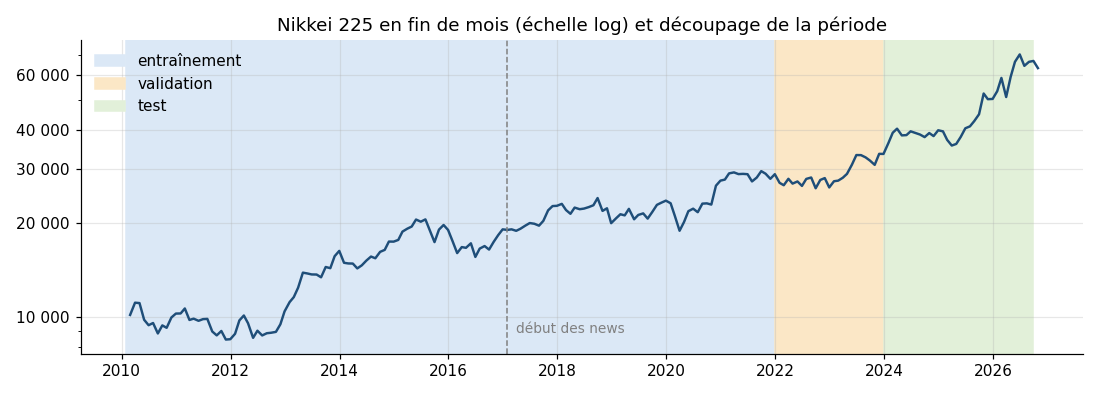
\includegraphics[width=.92\linewidth]{01_nikkei_split.png}
\caption{Nikkei 225 en fin de mois et découpage chronologique. Les news commencent en 2017.}
\end{figure}

L'exploration (notebook 01) fait ressortir deux faits qui guideront tout le projet : sur l'entraînement, le
\textbf{volume anormal d'articles} est la seule variable nettement liée au rendement du mois suivant (corrélation de
rang $-0{,}38$, $p=0{,}004$, 57 mois) ; et aucune variable ne prédit l'avantage de la couverture.

\begin{figure}[H]\centering
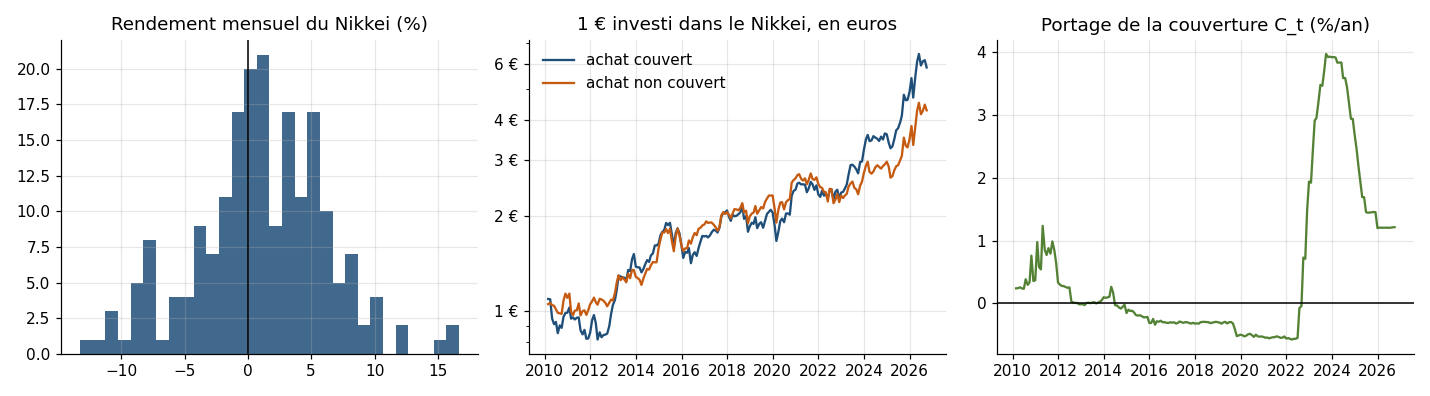
\includegraphics[width=\linewidth]{01_cibles_couverture.png}
\caption{Rendements mensuels du Nikkei (gauche), 1~\texteuro{} investi couvert ou non (milieu), portage de la couverture
(droite). Le portage, négatif de 2015 à 2021, devient fortement positif après 2022 : la couverture rapporte alors en
plus de protéger contre la baisse du yen.}
\end{figure}

Trois constats d'exploration ont un effet direct sur la modélisation. Le Nikkei monte 61~\% des mois, d'où un
déséquilibre modéré et une référence « toujours hausse » difficile à battre. Les news ne couvrent que 57 des 143 mois
d'entraînement, d'où l'imputation et l'indicateur de présence. Enfin, le portage change de signe entre l'entraînement
et le test : une variable qui garde la même pente sur un domaine aussi différent risque d'extrapoler, ce que la
section~\ref{sec:shap} confirme.

\section{Variables (exigence 2)}

Dix variables : momentum 3 et 12 mois, volatilité EWMA, variation du JGB 10 ans, Tankan, portage de la couverture
$C_t$, volatilité de l'EUR/JPY, et trois variables construites :
\[
A_t=\ln(n^J_t+n^B_t)-\tfrac16\textstyle\sum_{k=1}^{6}\ln(n^J_{t-k}+n^B_{t-k}),\qquad
\bar s_t=\frac{n^J_t s^J_t+n^B_t s^B_t}{n^J_t+n^B_t},\qquad \text{news\_dispo}_t=\mathbb 1\{A_t\text{ existe}\}
\]
($n$ : nombre d'articles Japon et BoJ ; $s$ : score FinBERT $P(\text{positif})-P(\text{négatif})$). S'y ajoutent, dans la
pipeline, les distances de chaque mois aux deux régimes d'un k-means (calme ou agité ; $k=2$ par le coude, L3B).
Avant 2017, les variables de news sont \textbf{manquantes} : elles sont imputées par la médiane de l'entraînement et
l'indicateur \texttt{news\_dispo} signale l'imputation. Aucune variable n'est catégorielle, il n'y a donc rien à encoder.

\section{Split, déséquilibre et pipeline (exigences 3 et 5)}

\begin{table}[H]\centering\small
\begin{tabular}{lcccp{4.4cm}}\toprule
Bloc & Période & Mois & Part de baisses & Rôle \\\midrule
Entraînement & 2010-02 → 2021-12 & 143 (57 avec news) & 39,2~\% & Optuna, \texttt{TimeSeriesSplit} 4 × 12 mois \\
Validation & 2022-01 → 2023-12 & 24 & 41,7~\% & choix du modèle \\
Test & 2024-01 → 2026-09 & 33 & 36,4~\% & une seule évaluation \\\bottomrule
\end{tabular}\end{table}

\textbf{Déséquilibre (exigence 3).} Il est modéré (39/61). Nous rapportons la PR-AUC, dont la référence vaut la
prévalence, la matrice de confusion avec les comptes, la precision, le recall et le F1 de la classe baisse, et non
l'accuracy (« toujours hausse » a 64~\% d'accuracy et un F1 nul sur le test). Deux remèdes du cours ont été comparés :
\texttt{class\_weight="balanced"} fait partie de l'espace de recherche d'Optuna, et le \textbf{seuil de décision}
(S7 : « changer le seuil, pas le modèle »). Optuna a gardé \texttt{class\_weight=None} pour les trois modèles : la
pondération tire les probabilités vers 50~\% et dégrade la log-loss, alors que la décision finale a besoin de
probabilités calibrées. Le remède retenu est donc le seuil, fixé par les coûts (section~\ref{sec:decision}). SMOTE est
écarté : il fabriquerait des mois synthétiques.

\textbf{Pipeline (exigence 5).} Une seule \texttt{Pipeline} scikit-learn : imputation, k-means (distances aux
centres), standardisation, modèle. Tout ce qui apprend un paramètre est réajusté dans chaque fold (S1, S3) ; un test
vérifie que les médianes d'imputation sont celles de l'entraînement et non celles de toutes les données.

\section{Trois modèles et réglage par Optuna (exigences 4, 6, 7)}

Régression logistique régularisée (solveur \texttt{saga}, qui ne pénalise pas l'intercept, contrairement à
\texttt{liblinear}), Random Forest et LightGBM ont été réglés par Optuna (50 essais chacun, TPE à graine fixe) en
minimisant la log-loss moyenne de 4 folds \texttt{TimeSeriesSplit} de 12 mois. Le score annoncé n'est pas celui
d'Optuna, qui est optimiste, mais celui de la validation puis du test. Les 200 essais sont journalisés dans
\texttt{runs/trials\_log.csv} (paramètres, log-loss par fold, Brier, PR-AUC, commit Git, modèle sauvegardé).

\begin{table}[H]\centering\small
\begin{tabular}{lccccc}\toprule
Modèle (Nikkei) & Log-loss CV & Log-loss validation & Brier validation & PR-AUC validation \\\midrule
Constant (référence) & 0,672 & \textbf{0,681} & \textbf{0,244} & 0,417 \\
Logistique & 0,647 & 0,701 & 0,253 & 0,489 \\
Random Forest & 0,629 & 0,742 & 0,273 & 0,440 \\
LightGBM & \textbf{0,584} & 0,710 & 0,257 & \textbf{0,524} \\\bottomrule
\end{tabular}
\caption{Les trois modèles battent la constante en validation croisée (98~\% des essais à arbres), aucun sur la validation.}
\end{table}

\textbf{Ce que chaque étape a apporté.} Les arbres captent des interactions qui marchent sur 2018-2021 mais ne se
transfèrent pas : plus le modèle est flexible, plus l'écart entre validation croisée et validation est grand. Deux
raisons : le réglage s'ajuste au bruit de 48 mois, et 2022-2023 est un autre régime (la BoJ desserre son contrôle des
taux, le portage redevient positif). Le modèle final est choisi par la \textbf{règle de baseline de S1} : on garde la
logistique, sauf si un modèle plus complexe la bat à la fois en PR-AUC et en log-loss calibrée sur la validation
(LightGBM classe mieux mais ses probabilités sont pires). Le modèle de couverture, lui, n'a aucun signal : le meilleur
réglage met tous ses coefficients à zéro, et la règle reste « toujours couvert ».

\begin{figure}[H]\centering
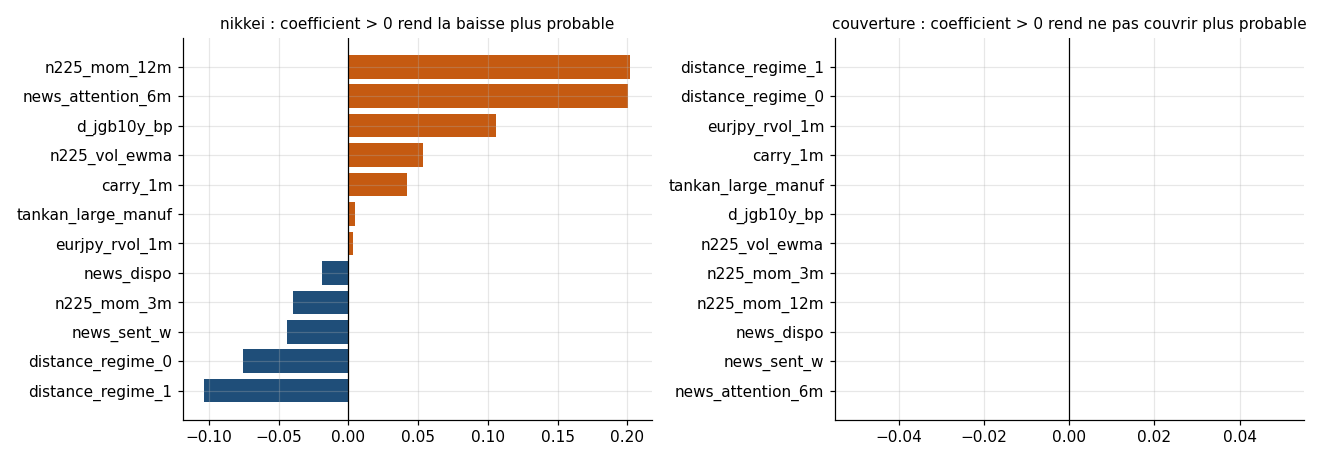
\includegraphics[width=.95\linewidth]{02_coefficients_logistiques.png}
\caption{Coefficients des régressions logistiques sur variables standardisées. Pour le Nikkei, un coefficient positif
rend la baisse plus probable ; le modèle de couverture n'a aucun coefficient non nul.}
\end{figure}

La logistique raconte la même histoire que l'exploration : un écart-type de plus sur le volume anormal d'articles
multiplie les odds de baisse par 1,22, comme un écart-type de plus sur le momentum 12 mois (lecture contrarienne), et
une hausse du JGB 10 ans par 1,11. Le sentiment FinBERT (× 0,96) et l'indicateur de présence des news (× 0,98) ne
pèsent presque rien, ce qui écarte le risque que cet indicateur, corrélé au portage, capte seulement l'époque.

\section{Calibration (exigence 9)}

La calibration de Platt, $p=\sigma(a f+c)$ avec $f$ le log-odds du modèle, est apprise sur les \textbf{prédictions
hors fold} 2018-2021. Un premier essai sur la validation donnait des pentes négatives : il inversait les modèles, appris
en échantillon, et a été écarté. Hors fold, la logistique est légèrement sur-confiante ($a=0{,}92$), le Random Forest
sous-confiant ($a=1{,}54$), LightGBM bien calibré ($a=0{,}99$).

\begin{figure}[H]\centering
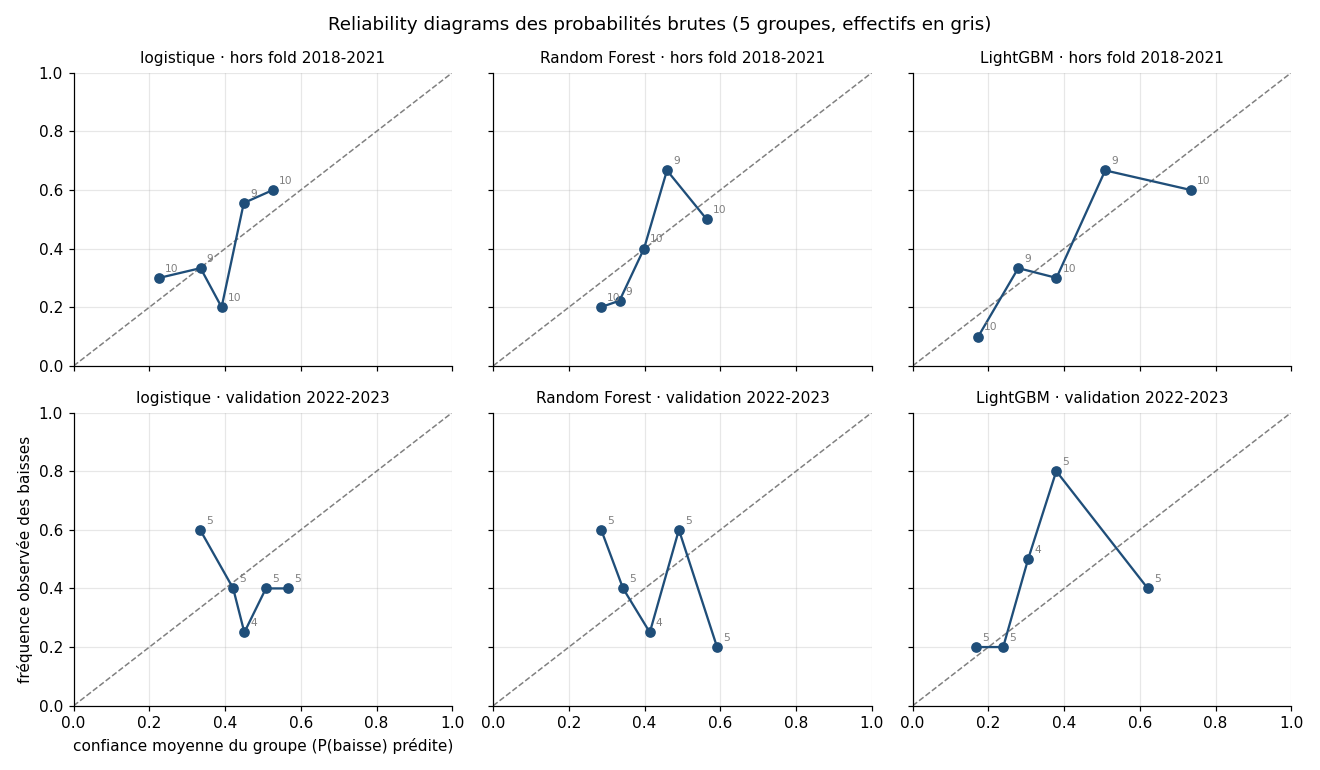
\includegraphics[width=.85\linewidth]{03_fiabilite_brute.png}
\caption{Reliability diagrams des probabilités brutes (5 groupes de même taille, effectifs en gris). Hors fold
(en haut), les points suivent à peu près la diagonale ; sur la validation (en bas), la courbe de la logistique
descend : plus le modèle annonce une baisse, moins elle arrive.}
\end{figure}

Sur la validation, la calibration ne sauve aucun modèle : la logistique calibrée garde une log-loss de 0,699 contre
0,681 pour la constante. Le diagnostic principal vient de l'exploration mois par mois : le volume anormal d'articles,
négativement corrélé au rendement suivant sur l'entraînement ($-0{,}38$), lui est positivement corrélé en 2022-2023
($+0{,}29$), au moment où les articles sur la BoJ passent de 55 à 73 par mois (ajustements du contrôle des taux,
changement de gouverneur).

\begin{figure}[H]\centering
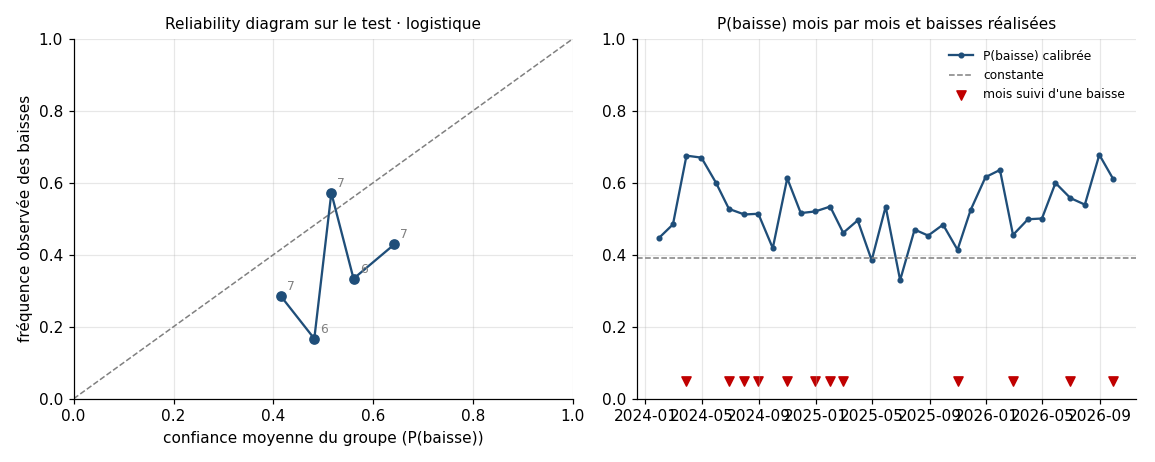
\includegraphics[width=.9\linewidth]{03b_test_probabilites.png}
\caption{Test 2024-2026. À gauche, quatre points sur cinq du reliability diagram sont sous la diagonale ; à droite,
la probabilité de baisse reste presque toujours au-dessus de la constante.}
\end{figure}

\textbf{Verdict sur le test.} Brier 0,257 contre 0,232 pour la constante, ECE 0,183 contre 0,144. Le modèle est
\textbf{sur-confiant dans la baisse} : 52~\% de baisses annoncées en moyenne pour 36~\% observées. Nous ne ferions pas
confiance à ces probabilités, telles quelles, pour une décision.

\section{Du score à la décision}\label{sec:decision}

Avec la probabilité calibrée de hausse $p_t$ et des rendements moyens mesurés \textbf{sur l'entraînement} (en excès du
cash : achat couvert $B_u=+3{,}89~\%$ un mois de hausse, $B_d=-4{,}18~\%$ un mois de baisse ; vente $S_u=-3{,}89~\%$,
$S_d=+4{,}18~\%$), on prend la position dont le gain espéré au-dessus du cash dépasse une marge $m$, sinon on reste neutre :
\[
\text{acheter si } p_t\ge\theta_a=\frac{m-B_d}{B_u-B_d},\qquad \text{vendre si } p_t\le\theta_v=\frac{S_d-m}{S_d-S_u},\qquad S_t=2p_t-1 .
\]
La marge est \textbf{fixée à l'avance} ($m=0{,}5~\%$ par mois, environ 6~\% par an) : $\theta_v=0{,}456$ et
$\theta_a=0{,}580$. Le F1 est rapporté mais ne sert pas à décider : il pousse à vendre souvent, alors qu'une fausse
alerte coûte cher sur un indice qui monte 61~\% des mois. Le modèle, la calibration, les coûts, la marge et la
couverture ont été \textbf{figés et commités} (\texttt{runs/decision\_finale.json}, commit \texttt{0d8df2f}) avant toute
évaluation sur le test, avec un engagement : si le modèle y perd contre la constante, recommander « toujours acheter,
couvert ».

\section{Évaluation unique sur le test 2024-2026}

\begin{table}[H]\centering\small
\begin{tabular}{lcccc}\toprule
 & Log-loss & PR-AUC & Rendement cumulé en € & Perte maximale \\\midrule
Logistique calibrée, règle de décision & 0,708 & 0,420 & +3,5~\% & $-23$~\% \\
Modèle constant & \textbf{0,657} & 0,364 & & \\
Toujours acheter, couvert & & & \textbf{+82,3~\%} & $-13$~\% \\
Toujours acheter, non couvert & & & +57,9~\% & $-13$~\% \\\bottomrule
\end{tabular}\end{table}

Au seuil 0,5, le F1 de la classe baisse vaut 0,563 (TP 9, FP 11, FN 3, TN 10), à peine au-dessus de « toujours
baisse » (0,533). La règle donne 4 achats, 19 mois neutres et 10 ventes : elle évite 11 baisses sur 12, mais reste
hors du marché pendant 18 hausses. \textbf{Le plancher n'est pas battu} ; conformément à l'engagement, la
recommandation est \emph{« toujours acheter, couvert »}. La couverture permanente, elle, était le bon choix (meilleure
61~\% des mois).

\begin{figure}[H]\centering
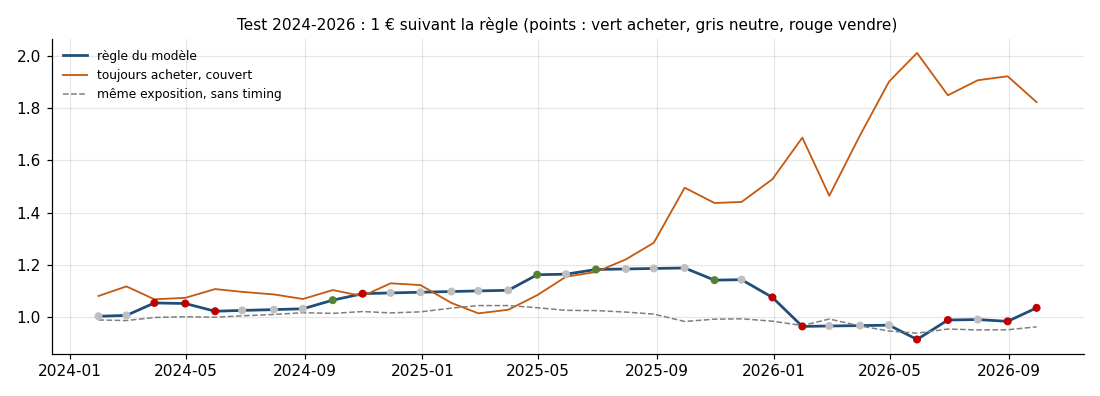
\includegraphics[width=.95\linewidth]{03b_test_regle.png}
\caption{1~\texteuro{} suivant la règle sur le test (points : vert acheter, gris neutre, rouge vendre), contre « toujours
acheter, couvert » et la même exposition moyenne sans timing.}
\end{figure}

Face à la référence honnête, la même exposition moyenne sans aucun timing ($-3{,}7~\%$), le choix du moment rapporte à
peine 7 points : le modèle a un faible signal de classement (PR-AUC au-dessus du hasard sur la validation comme sur le
test), mais il est trop pessimiste pour être utile dans un marché qui monte durablement. Seule l'année 2024 fait
exception : le modèle y bat la constante (log-loss 0,672 contre 0,717) et détecte les 6 baisses de l'année.

\section{Explicabilité et diagnostics (exigence 8)}\label{sec:shap}

\begin{figure}[H]\centering
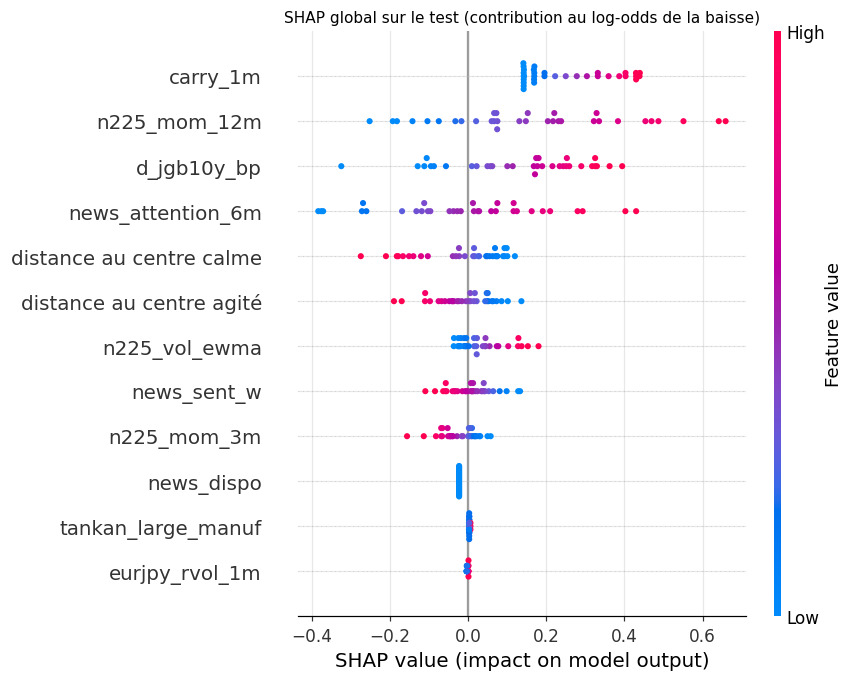
\includegraphics[width=.47\linewidth]{04_shap_beeswarm_test.png}\hfill
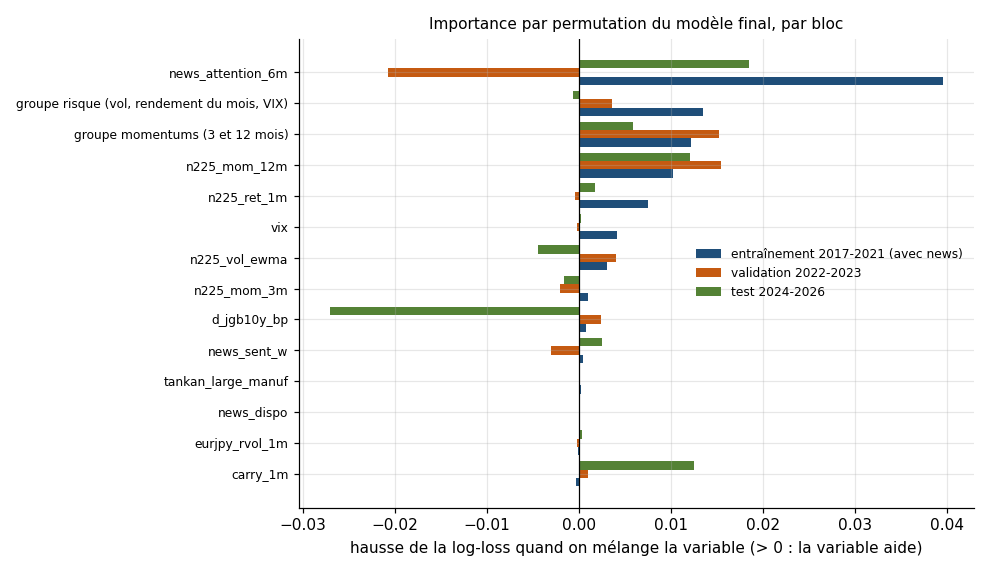
\includegraphics[width=.5\linewidth]{04_permutation.png}
\caption{À gauche, SHAP sur le test (contribution au log-odds de la baisse). À droite, importance par permutation sur
2017-2021, la validation et le test.}
\end{figure}

\begin{itemize}
\item \textbf{Ce que le modèle a appris.} Le volume anormal d'articles est la variable la plus utile à l'entraînement
(la log-loss monte de 0,040 quand on la mélange), puis le risque et les momentums. Le sentiment FinBERT ne pèse
presque rien.
\item \textbf{Ce qui a cassé.} Le signal des news est \textbf{instable} : il nuit sur la validation mais aide de nouveau
sur le test, et sa corrélation glissante sur 24 mois oscille entre $-0{,}5$ et $+0{,}3$. Sur le test, trois variables
poussent vers « baisse » (SHAP signé) : le portage (+0,25), qui est à 6 écarts-types de sa moyenne d'entraînement
(extrapolation), le momentum 12 mois (+0,17), pari contrarien contre une tendance durable, et la hausse du JGB (+0,13),
alors que la BoJ remonte ses taux pendant que le marché monte.
\item \textbf{Sens économique.} Un pic d'articles traduisait du stress jusqu'en 2021, puis une normalisation monétaire ;
le momentum contrarien convenait aux rebonds en V de 2018-2021, pas à une tendance longue. SHAP décrit le modèle, pas
l'économie : il n'établit aucune causalité (S9).
\item \textbf{Explication locale.} Fin juillet 2024, avant le krach du 5 août, le modèle donne 51~\% de baisse : le
portage pousse à lui seul de +0,40 en log-odds, la baisse récente du JGB retire 0,11. Le Nikkei a fini le mois à
$-1{,}2~\%$. Fin octobre 2026, le dernier mois, le modèle donne 45~\% de hausse et sa règle dirait « vendre », poussée
surtout par un pic d'articles ; la collecte des news de fin 2026 étant incomplète, ce signal est fragile.
\item \textbf{Une leçon de méthode.} L'importance par permutation ne voit pas un décalage de niveau, puisqu'elle mélange
des valeurs toutes élevées ; SHAP, qui compare chaque mois à la moyenne de l'entraînement, le voit.
\end{itemize}

\begin{figure}[H]\centering
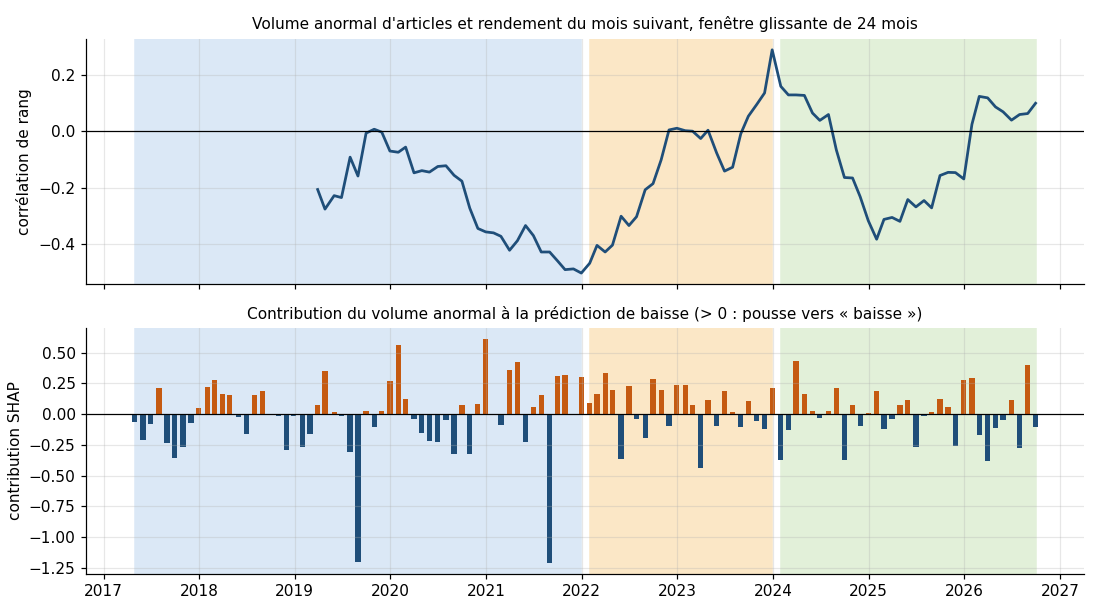
\includegraphics[width=.92\linewidth]{04_inversion_signal_news.png}
\caption{En haut, corrélation de rang glissante (24 mois) entre le volume anormal d'articles et le rendement du mois
suivant ; en bas, contribution SHAP de cette variable à la prédiction de baisse. Bleu : entraînement ; orange :
validation ; vert : test.}
\end{figure}

\section{Équité et biais (exigence 10)}

Le jeu ne contient \textbf{aucune personne}, donc aucun attribut sensible au sens de l'énoncé : les définitions
d'équité entre groupes de personnes ne s'appliquent pas, et nous ne prétendons pas les avoir satisfaites. Nous
transposons la démarche à des \textbf{groupes de mois} pour lesquels une inégalité de traitement aurait un coût
(slices de S9, test 2024-2026, seuil 0,5) :

\begin{table}[H]\centering\small
\begin{tabular}{lcccccc}\toprule
Groupe & Mois & Baisses & Recall\textsuperscript{a} & Faux positifs\textsuperscript{b} & Log-loss & Log-loss constante \\\midrule
Régime calme & 24 & 9 & 0,78 & 0,60 & 0,725 & 0,662 \\
Régime agité & 9 & 3 & 0,67 & 0,33 & 0,660 & 0,644 \\
Réunion BoJ le mois suivant & 22 & 8 & 0,75 & 0,50 & 0,690 & 0,657 \\
Pas de réunion BoJ & 11 & 4 & 0,75 & 0,57 & 0,743 & 0,657 \\\bottomrule
\end{tabular}
\caption*{\small a. Recall de la classe baisse, l'« égalité des chances ». b. Taux de faux positifs. Seuil 0,5, test 2024-2026.}\end{table}

L'écart de recall entre régimes (0,11) est bien inférieur à son erreur type (0,14 à 0,27 avec 3 à 9 baisses par
groupe) : rien ne permet de conclure à un traitement inégal. L'écart de taux de faux positifs (0,27) et de parité
(0,22, part de mois prédits en baisse) est plus net.

\paragraph{Mitigation : repondération (Kamiran et Calders).} Attribut : le régime k-means. Nous réentraînons la même
pipeline, avec les mêmes hyperparamètres, en pondérant chaque mois d'entraînement par $w(g,y)=P(g)P(y)/P(g,y)$, ce qui
rend régime et cible indépendants dans les données d'apprentissage ; la calibration de Platt est réapprise comme pour
le modèle figé, sur les prédictions hors fold de l'entraînement. Rien n'est réglé sur le test, comparé avant et après
(\texttt{python -m src.equite}, \texttt{runs/equite\_mitigation.json}). Ce calcul est postérieur à l'ouverture du
test et ne change pas la décision figée.

\begin{table}[H]\centering\footnotesize\setlength\tabcolsep{4pt}
\begin{tabular}{lccccccc}\toprule
Test 2024-2026 & Recall calme & Recall agité & Écart recall & Écart FP & Écart parité & Log-loss & Exactitude \\\midrule
Avant (modèle figé) & 0,78 & 0,67 & 0,11 & 0,27 & 0,22 & 0,708 & 0,58 \\
Après repondération & 0,56 & 0,67 & 0,11 & 0,03 & 0,01 & 0,700 & 0,52 \\\bottomrule
\end{tabular}
\caption*{\small Seuil 0,5, classe positive : la baisse. Log-loss du modèle constant sur le test : 0,657.}\end{table}

La repondération égalise presque les taux de faux positifs et la parité entre régimes, et améliore un peu la log-loss,
au prix de 6 points d'exactitude : le modèle prédit moins souvent la baisse en régime calme. L'égalité des chances
(écart de recall) ne bouge pas, et avec 3 baisses en régime agité aucun de ces écarts n'est significatif. Sur la
seconde version (Bloomberg, 1999-2026), le même audit donne un recall de 0,18 en régime calme (11 baisses) contre
1,00 en régime agité, mais sur \emph{une seule} baisse ; régime et cible y sont déjà presque indépendants à
l'entraînement (poids entre 0,96 et 1,03), si bien que la repondération ne change rien. Conclusion : nous ne
retiendrions pas cette mitigation, dont l'effet ne se distingue pas du bruit, et l'équité reste la principale limite du
projet au regard de l'énoncé, faute d'attribut sensible au sens propre.

% Section prête à insérer dans rapport.tex, juste avant « \section{Limites} », avec : % Section prête à insérer dans rapport.tex, juste avant « \section{Limites} », avec : % Section prête à insérer dans rapport.tex, juste avant « \section{Limites} », avec : \input{section_apres_coup}
% Elle n'est pas encore incluse : le rapport n'a pas pu être recompilé sur cette machine (pas de LaTeX installé).
% Tous les chiffres viennent de runs/exploration_*.json (python -m src.banc_essai, src.banc_essai_jour,
% src.banc_essai_long, src.volatilite).

\section{Après le test : vérifications et second volet}

Tout ce qui suit a été fait \textbf{après} l'ouverture du test. Ces essais éclairent le résultat de la section
précédente ; ils ne le remplacent pas, et les fichiers figés n'ont pas été modifiés.

\paragraph{Un autre modèle aurait-il fait mieux ?} Nous avons réentraîné chaque mois vingt modèles (logistiques,
forêts, LightGBM, réseau de neurones, AR(1), lissage exponentiel\ldots), sur tout le passé ou sur les 60 derniers mois.
Sur les 33 mois du test, 3 configurations sur 38 passent sous la log-loss de la constante, avec une avance
($-0{,}009 \pm 0{,}039$ pour la meilleure) quatre fois plus petite que son erreur type. Le modèle le mieux classé sur
2016-2023 (15 plus proches voisins) finit parmi les moins bons sur le test. Sur la base journalière (4\,118 séances),
l'AUC du sens du lendemain vaut 0,49 sur 668 séances de test. Faire commencer l'apprentissage en 2000 plutôt qu'en 2010
dégrade la constante (0,667 contre 0,660). Le blocage vient donc de l'information disponible, pas du choix du modèle.

\paragraph{Un piège d'horaires.} Dans la base journalière, la ligne d'un jour contient la clôture de Wall Street du
même jour, connue après celle de Tokyo. L'utiliser telle quelle donne une AUC de 0,71, sans décision possible derrière.
Toutes les séries étrangères ont donc été décalées d'un jour.

\paragraph{Second volet : prévoir l'agitation.} Avec les mêmes mois, le même découpage et un réentraînement mensuel,
nous avons changé de cible : la volatilité réalisée du mois suivant, et la classe « mois agité » (volatilité au-dessus
de 20~\%).

\begin{table}[H]\centering\small
\begin{tabular}{lcc}\toprule
 & 2016-2023 (95 mois) & Test 2024-2026 (33 mois) \\\midrule
Volatilité : $R^2$ hors échantillon, régression (vol. 1, 3, 6 mois, VIX, rendement) & 0,23 & 0,18 \\
Volatilité : $R^2$ hors échantillon, GARCH(1,1) & 0,03 & 0,32 \\
Mois agité : AUC de la régression logistique & 0,73 & 0,71 \\
Mois agité : écart de log-loss avec la constante & $-0{,}074 \pm 0{,}041$ & $-0{,}065 \pm 0{,}088$ \\\bottomrule
\end{tabular}\end{table}

Le classement des mois est stable d'une période à l'autre (AUC proche de 0,7, contre 0,5 pour le sens du marché),
mais sur 33 mois l'avantage en log-loss reste inférieur à son erreur type, et le classement des méthodes de
prévision change selon la période. Une position dosée selon la volatilité prévue (part investie $= 15~\%/\hat\sigma$,
plafonnée à 100~\%) ramène le pire mois de $-13{,}2~\%$ à $-9{,}7~\%$ et le rendement de $+82{,}3~\%$ à $+67{,}7~\%$ :
rapporté au risque, le résultat est le même (1,00 contre 0,98). Ce volet sert à annoncer le risque ; il ne fournit pas
une stratégie meilleure que « toujours acheter, couvert ».

% Elle n'est pas encore incluse : le rapport n'a pas pu être recompilé sur cette machine (pas de LaTeX installé).
% Tous les chiffres viennent de runs/exploration_*.json (python -m src.banc_essai, src.banc_essai_jour,
% src.banc_essai_long, src.volatilite).

\section{Après le test : vérifications et second volet}

Tout ce qui suit a été fait \textbf{après} l'ouverture du test. Ces essais éclairent le résultat de la section
précédente ; ils ne le remplacent pas, et les fichiers figés n'ont pas été modifiés.

\paragraph{Un autre modèle aurait-il fait mieux ?} Nous avons réentraîné chaque mois vingt modèles (logistiques,
forêts, LightGBM, réseau de neurones, AR(1), lissage exponentiel\ldots), sur tout le passé ou sur les 60 derniers mois.
Sur les 33 mois du test, 3 configurations sur 38 passent sous la log-loss de la constante, avec une avance
($-0{,}009 \pm 0{,}039$ pour la meilleure) quatre fois plus petite que son erreur type. Le modèle le mieux classé sur
2016-2023 (15 plus proches voisins) finit parmi les moins bons sur le test. Sur la base journalière (4\,118 séances),
l'AUC du sens du lendemain vaut 0,49 sur 668 séances de test. Faire commencer l'apprentissage en 2000 plutôt qu'en 2010
dégrade la constante (0,667 contre 0,660). Le blocage vient donc de l'information disponible, pas du choix du modèle.

\paragraph{Un piège d'horaires.} Dans la base journalière, la ligne d'un jour contient la clôture de Wall Street du
même jour, connue après celle de Tokyo. L'utiliser telle quelle donne une AUC de 0,71, sans décision possible derrière.
Toutes les séries étrangères ont donc été décalées d'un jour.

\paragraph{Second volet : prévoir l'agitation.} Avec les mêmes mois, le même découpage et un réentraînement mensuel,
nous avons changé de cible : la volatilité réalisée du mois suivant, et la classe « mois agité » (volatilité au-dessus
de 20~\%).

\begin{table}[H]\centering\small
\begin{tabular}{lcc}\toprule
 & 2016-2023 (95 mois) & Test 2024-2026 (33 mois) \\\midrule
Volatilité : $R^2$ hors échantillon, régression (vol. 1, 3, 6 mois, VIX, rendement) & 0,23 & 0,18 \\
Volatilité : $R^2$ hors échantillon, GARCH(1,1) & 0,03 & 0,32 \\
Mois agité : AUC de la régression logistique & 0,73 & 0,71 \\
Mois agité : écart de log-loss avec la constante & $-0{,}074 \pm 0{,}041$ & $-0{,}065 \pm 0{,}088$ \\\bottomrule
\end{tabular}\end{table}

Le classement des mois est stable d'une période à l'autre (AUC proche de 0,7, contre 0,5 pour le sens du marché),
mais sur 33 mois l'avantage en log-loss reste inférieur à son erreur type, et le classement des méthodes de
prévision change selon la période. Une position dosée selon la volatilité prévue (part investie $= 15~\%/\hat\sigma$,
plafonnée à 100~\%) ramène le pire mois de $-13{,}2~\%$ à $-9{,}7~\%$ et le rendement de $+82{,}3~\%$ à $+67{,}7~\%$ :
rapporté au risque, le résultat est le même (1,00 contre 0,98). Ce volet sert à annoncer le risque ; il ne fournit pas
une stratégie meilleure que « toujours acheter, couvert ».

% Elle n'est pas encore incluse : le rapport n'a pas pu être recompilé sur cette machine (pas de LaTeX installé).
% Tous les chiffres viennent de runs/exploration_*.json (python -m src.banc_essai, src.banc_essai_jour,
% src.banc_essai_long, src.volatilite).

\section{Après le test : vérifications et second volet}

Tout ce qui suit a été fait \textbf{après} l'ouverture du test. Ces essais éclairent le résultat de la section
précédente ; ils ne le remplacent pas, et les fichiers figés n'ont pas été modifiés.

\paragraph{Un autre modèle aurait-il fait mieux ?} Nous avons réentraîné chaque mois vingt modèles (logistiques,
forêts, LightGBM, réseau de neurones, AR(1), lissage exponentiel\ldots), sur tout le passé ou sur les 60 derniers mois.
Sur les 33 mois du test, 3 configurations sur 38 passent sous la log-loss de la constante, avec une avance
($-0{,}009 \pm 0{,}039$ pour la meilleure) quatre fois plus petite que son erreur type. Le modèle le mieux classé sur
2016-2023 (15 plus proches voisins) finit parmi les moins bons sur le test. Sur la base journalière (4\,118 séances),
l'AUC du sens du lendemain vaut 0,49 sur 668 séances de test. Faire commencer l'apprentissage en 2000 plutôt qu'en 2010
dégrade la constante (0,667 contre 0,660). Le blocage vient donc de l'information disponible, pas du choix du modèle.

\paragraph{Un piège d'horaires.} Dans la base journalière, la ligne d'un jour contient la clôture de Wall Street du
même jour, connue après celle de Tokyo. L'utiliser telle quelle donne une AUC de 0,71, sans décision possible derrière.
Toutes les séries étrangères ont donc été décalées d'un jour.

\paragraph{Second volet : prévoir l'agitation.} Avec les mêmes mois, le même découpage et un réentraînement mensuel,
nous avons changé de cible : la volatilité réalisée du mois suivant, et la classe « mois agité » (volatilité au-dessus
de 20~\%).

\begin{table}[H]\centering\small
\begin{tabular}{lcc}\toprule
 & 2016-2023 (95 mois) & Test 2024-2026 (33 mois) \\\midrule
Volatilité : $R^2$ hors échantillon, régression (vol. 1, 3, 6 mois, VIX, rendement) & 0,23 & 0,18 \\
Volatilité : $R^2$ hors échantillon, GARCH(1,1) & 0,03 & 0,32 \\
Mois agité : AUC de la régression logistique & 0,73 & 0,71 \\
Mois agité : écart de log-loss avec la constante & $-0{,}074 \pm 0{,}041$ & $-0{,}065 \pm 0{,}088$ \\\bottomrule
\end{tabular}\end{table}

Le classement des mois est stable d'une période à l'autre (AUC proche de 0,7, contre 0,5 pour le sens du marché),
mais sur 33 mois l'avantage en log-loss reste inférieur à son erreur type, et le classement des méthodes de
prévision change selon la période. Une position dosée selon la volatilité prévue (part investie $= 15~\%/\hat\sigma$,
plafonnée à 100~\%) ramène le pire mois de $-13{,}2~\%$ à $-9{,}7~\%$ et le rendement de $+82{,}3~\%$ à $+67{,}7~\%$ :
rapporté au risque, le résultat est le même (1,00 contre 0,98). Ce volet sert à annoncer le risque ; il ne fournit pas
une stratégie meilleure que « toujours acheter, couvert ».


\section{Limites}

\begin{itemize}
\item \textbf{Petit échantillon} : 143 mois d'entraînement, 12 baisses dans le test.
\item \textbf{Test pas entièrement invisible} : l'exploration affichait déjà des statistiques du bloc test (part de baisses,
courbe « achat couvert ou non ») avant le gel ; la couverture permanente et la règle de repli n'ont pas été choisies à
l'aveugle. Les variables ont été choisies à partir d'une analyse de 2017-2026.
\item \textbf{Fold de calibration imparfait} : Platt est appris sur les folds qui ont servi au réglage.
\item \textbf{Régime qui change} : les variables de taux sortent de leur domaine d'entraînement après 2022.
\item \textbf{Pistes, non testées} : standardiser sur une fenêtre glissante, borner ou retirer les variables de taux,
recalibrer en continu, signal de news à fréquence quotidienne. Elles ne pourront être jugées que sur des données
postérieures à septembre 2026.
\end{itemize}

\section{Code, reproductibilité et plateforme}

Le code principal est en Python (\texttt{src/}) : construction de la table et audit, pipeline, réglage, décision,
évaluation, prédiction, régression logistique codée à la main. Toutes les graines sont fixées ; deux exécutions du
réglage donnent les mêmes 200 essais ; \texttt{python -m src.decision --verifier} et \texttt{python -m src.evaluate
--verifier} retrouvent les fichiers figés à l'identique sans les réécrire ; 28 tests passent. Une API FastAPI sert le
signal (\texttt{/signal}, \texttt{/explication}, \texttt{/historique}, \texttt{/evaluation}) et un tableau de bord
Streamlit le présente. Les notebooks sont du matériel complémentaire ; le notebook 09 rassemble tout le code avec les concepts expliqués. La partie mathématique fait l'objet d'un rapport séparé (\texttt{report/rapport\_maths.tex}).

% Rôles des membres et usage de l'IA : partie commune aux deux rapports (% Rôles des membres et usage de l'IA : partie commune aux deux rapports (% Rôles des membres et usage de l'IA : partie commune aux deux rapports (\input{roles_et_ia}).

\section*{Contributions des membres}

\begin{table}[H]\centering\small
\begin{tabular}{p{3.2cm}p{12cm}}\toprule
Membre & Ce qu'il a fait \\\midrule
\textbf{Yann Linganzi} &
\textbf{Conception et conduite du projet.} Choix de la question (acheter, rester neutre ou vendre le Nikkei, couvert
ou non contre le yen) et de sa traduction en deux classifications ; collecte des données (versions 1 et 2), choix des
sources et des décalages de publication ; audit des fuites ; exploration et construction des variables ; découpage
chronologique ; pipeline, trois modèles et réglage Optuna ; choix de la log-loss comme critère ; calibration de Platt
et règle de décision par espérance de gain, figées avant le test ; évaluation unique du test ; explicabilité
(tranches, permutation, SHAP, dépendances partielles) ; annexe mathématique (logistique codée à la main, sensibilité,
moindres carrés) ; seconde version 1999-2026 avec le contrôle des séries Bloomberg ; explorations après coup et
protocole figé de la troisième version ; API, tableau de bord et site ; rédaction des rapports. \\[3pt]
\textbf{arnshl} &
Captures du terminal Bloomberg (huit écrans : inflation japonaise, fondamentaux et décomposition du rendement du
Nikkei, révisions des bénéfices, rendement des bénéfices contre le taux américain à 10 ans, trajectoires du bénéfice
par action), avec les vérifications visuelles et les pistes de variables qu'elles suggèrent ; chiffres qui justifient
les conclusions des salles III et VII du site ; relecture et fusion des contributions sur GitHub. \\[3pt]
\textbf{jovi-mce} &
Version anglaise du site (\texttt{site/en/}) et sa mise en ligne. \\\bottomrule
\end{tabular}\end{table}

\section*{Usage de l'IA}

La réflexion et la méthode sont les nôtres. Yann Linganzi a posé le problème et décidé de chaque choix de méthode :
les variables et leurs dates de publication, le découpage dans le temps, les modèles comparés, le critère, la
calibration, la règle de décision et l'engagement pris avant d'ouvrir le test, puis, après coup, les vérifications à
mener et le protocole de la troisième version. Il a testé chacun de ces choix et validé chaque résultat : audit des
fuites, vérifications qui retrouvent à l'identique la décision et l'évaluation figées, tests automatiques, lecture et
interprétation des chiffres.

Un assistant IA (Claude, d'Anthropic) a servi d'aide à la programmation : écriture du code Python des modules et des
notebooks à partir de ces choix, mise en forme du site et des figures, et aide à la relecture et à la mise en forme de
la rédaction. Tout ce qu'il a produit a été relu, exécuté et vérifié avant d'être gardé ; quand un résultat ne
tenait pas, c'est la méthode qui a été corrigée, pas le chiffre. La soutenance est assurée par le groupe.
).

\section*{Contributions des membres}

\begin{table}[H]\centering\small
\begin{tabular}{p{3.2cm}p{12cm}}\toprule
Membre & Ce qu'il a fait \\\midrule
\textbf{Yann Linganzi} &
\textbf{Conception et conduite du projet.} Choix de la question (acheter, rester neutre ou vendre le Nikkei, couvert
ou non contre le yen) et de sa traduction en deux classifications ; collecte des données (versions 1 et 2), choix des
sources et des décalages de publication ; audit des fuites ; exploration et construction des variables ; découpage
chronologique ; pipeline, trois modèles et réglage Optuna ; choix de la log-loss comme critère ; calibration de Platt
et règle de décision par espérance de gain, figées avant le test ; évaluation unique du test ; explicabilité
(tranches, permutation, SHAP, dépendances partielles) ; annexe mathématique (logistique codée à la main, sensibilité,
moindres carrés) ; seconde version 1999-2026 avec le contrôle des séries Bloomberg ; explorations après coup et
protocole figé de la troisième version ; API, tableau de bord et site ; rédaction des rapports. \\[3pt]
\textbf{arnshl} &
Captures du terminal Bloomberg (huit écrans : inflation japonaise, fondamentaux et décomposition du rendement du
Nikkei, révisions des bénéfices, rendement des bénéfices contre le taux américain à 10 ans, trajectoires du bénéfice
par action), avec les vérifications visuelles et les pistes de variables qu'elles suggèrent ; chiffres qui justifient
les conclusions des salles III et VII du site ; relecture et fusion des contributions sur GitHub. \\[3pt]
\textbf{jovi-mce} &
Version anglaise du site (\texttt{site/en/}) et sa mise en ligne. \\\bottomrule
\end{tabular}\end{table}

\section*{Usage de l'IA}

La réflexion et la méthode sont les nôtres. Yann Linganzi a posé le problème et décidé de chaque choix de méthode :
les variables et leurs dates de publication, le découpage dans le temps, les modèles comparés, le critère, la
calibration, la règle de décision et l'engagement pris avant d'ouvrir le test, puis, après coup, les vérifications à
mener et le protocole de la troisième version. Il a testé chacun de ces choix et validé chaque résultat : audit des
fuites, vérifications qui retrouvent à l'identique la décision et l'évaluation figées, tests automatiques, lecture et
interprétation des chiffres.

Un assistant IA (Claude, d'Anthropic) a servi d'aide à la programmation : écriture du code Python des modules et des
notebooks à partir de ces choix, mise en forme du site et des figures, et aide à la relecture et à la mise en forme de
la rédaction. Tout ce qu'il a produit a été relu, exécuté et vérifié avant d'être gardé ; quand un résultat ne
tenait pas, c'est la méthode qui a été corrigée, pas le chiffre. La soutenance est assurée par le groupe.
).

\section*{Contributions des membres}

\begin{table}[H]\centering\small
\begin{tabular}{p{3.2cm}p{12cm}}\toprule
Membre & Ce qu'il a fait \\\midrule
\textbf{Yann Linganzi} &
\textbf{Conception et conduite du projet.} Choix de la question (acheter, rester neutre ou vendre le Nikkei, couvert
ou non contre le yen) et de sa traduction en deux classifications ; collecte des données (versions 1 et 2), choix des
sources et des décalages de publication ; audit des fuites ; exploration et construction des variables ; découpage
chronologique ; pipeline, trois modèles et réglage Optuna ; choix de la log-loss comme critère ; calibration de Platt
et règle de décision par espérance de gain, figées avant le test ; évaluation unique du test ; explicabilité
(tranches, permutation, SHAP, dépendances partielles) ; annexe mathématique (logistique codée à la main, sensibilité,
moindres carrés) ; seconde version 1999-2026 avec le contrôle des séries Bloomberg ; explorations après coup et
protocole figé de la troisième version ; API, tableau de bord et site ; rédaction des rapports. \\[3pt]
\textbf{arnshl} &
Captures du terminal Bloomberg (huit écrans : inflation japonaise, fondamentaux et décomposition du rendement du
Nikkei, révisions des bénéfices, rendement des bénéfices contre le taux américain à 10 ans, trajectoires du bénéfice
par action), avec les vérifications visuelles et les pistes de variables qu'elles suggèrent ; chiffres qui justifient
les conclusions des salles III et VII du site ; relecture et fusion des contributions sur GitHub. \\[3pt]
\textbf{jovi-mce} &
Version anglaise du site (\texttt{site/en/}) et sa mise en ligne. \\\bottomrule
\end{tabular}\end{table}

\section*{Usage de l'IA}

La réflexion et la méthode sont les nôtres. Yann Linganzi a posé le problème et décidé de chaque choix de méthode :
les variables et leurs dates de publication, le découpage dans le temps, les modèles comparés, le critère, la
calibration, la règle de décision et l'engagement pris avant d'ouvrir le test, puis, après coup, les vérifications à
mener et le protocole de la troisième version. Il a testé chacun de ces choix et validé chaque résultat : audit des
fuites, vérifications qui retrouvent à l'identique la décision et l'évaluation figées, tests automatiques, lecture et
interprétation des chiffres.

Un assistant IA (Claude, d'Anthropic) a servi d'aide à la programmation : écriture du code Python des modules et des
notebooks à partir de ces choix, mise en forme du site et des figures, et aide à la relecture et à la mise en forme de
la rédaction. Tout ce qu'il a produit a été relu, exécuté et vérifié avant d'être gardé ; quand un résultat ne
tenait pas, c'est la méthode qui a été corrigée, pas le chiffre. La soutenance est assurée par le groupe.


\appendix
\section{Journal des essais (exigence 7)}

Le journal complet est le fichier \texttt{runs/trials\_log.csv} du dépôt (200 lignes : modèle, numéro d'essai,
paramètres, log-loss moyenne et par fold, Brier, PR-AUC, commit, modèle sauvegardé). Les essais retenus :

\begin{table}[H]\centering\small
\begin{tabular}{llcp{8.2cm}}\toprule
Cible & Modèle & Log-loss CV & Paramètres retenus \\\midrule
Nikkei & Logistique & 0,6473 & L2, $C=0{,}030$, sans pondération \\
Nikkei & Random Forest & 0,6288 & 100 arbres, profondeur 4, 5 mois par feuille, \texttt{max\_features}=0,5 \\
Nikkei & LightGBM & 0,5836 & 75 arbres, learning rate 0,067, 7 feuilles, 6 mois par feuille, $\lambda=1{,}84$ \\
Couverture & Logistique & 0,6875 & L1, $C=0{,}0035$, pondération \texttt{balanced} (tous les coefficients nuls) \\\bottomrule
\end{tabular}\end{table}

\begin{figure}[H]\centering
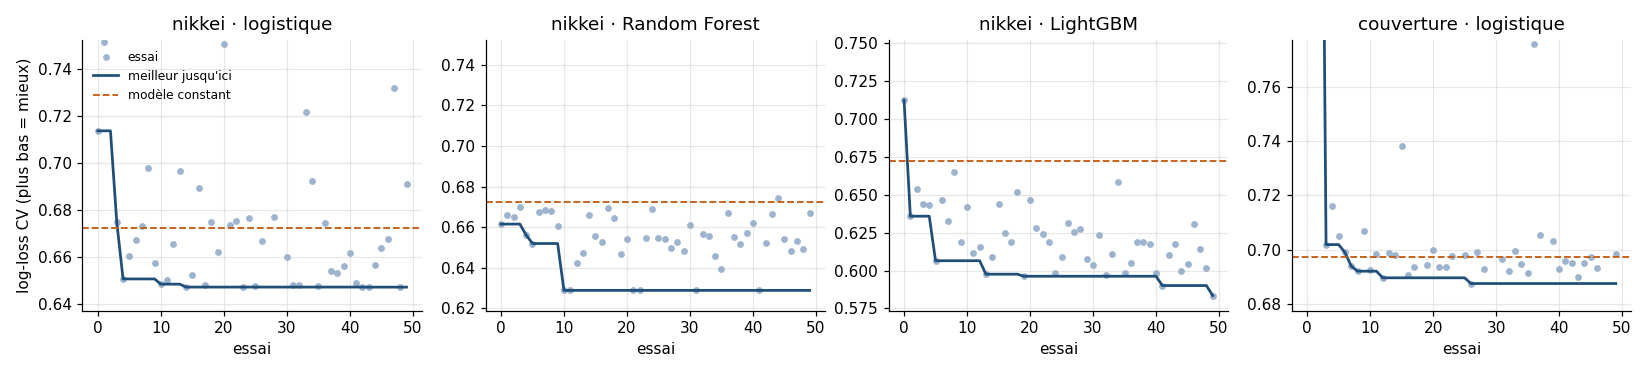
\includegraphics[width=\linewidth]{02_optuna_historique.png}
\caption{Historique des essais Optuna : log-loss de chaque essai, meilleur jusqu'ici, et modèle constant.}
\end{figure}

\end{document}
